\chapter{Dise\~no Detallado}
\section{Electroimanes}
Para dise�ar un electroim�n se requiere de un modelo que relacione la geometr�a del n�cleo con la fuerza m�xima que este puede ejercer. Sabemos por la ecuaci�n ?? que la fuerza esta determinada por
\begin{equation}
	F =  \frac{(NI)^2}{2} \frac{d}{dy}(\mathcal{R}^{-1})
\end{equation}
por lo que el problema de calcular la fuerza se reduce a calcular la reluctancia del circuito magn�tico que conforma el electroim�n. Procederemos a analizar los n�cleos de geometr�a \ref{fig:geometria-radial} y \ref{fig:geometria-axial} correspondientes a los electroimanes radial y axial respectivamente.

\begin{figure}[htb]
    \centering
    \begin{subfigure}[b]{0.4\textwidth}
        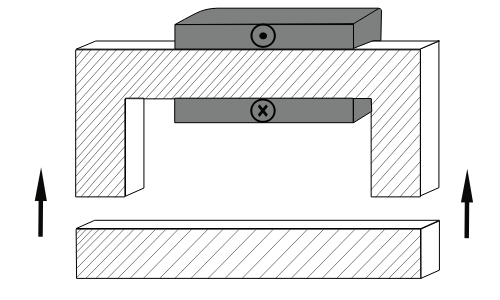
\includegraphics[width=\textwidth]{images/Capitulo_2/geometria_nucleo_axial}
        \caption{radial}
        \label{fig:geometria-radial}
    \end{subfigure}
    ~ %add desired spacing between images, e. g. ~, \quad, \qquad, \hfill etc. 
      %(or a blank line to force the subfigure onto a new line)
    \begin{subfigure}[b]{0.4\textwidth}
        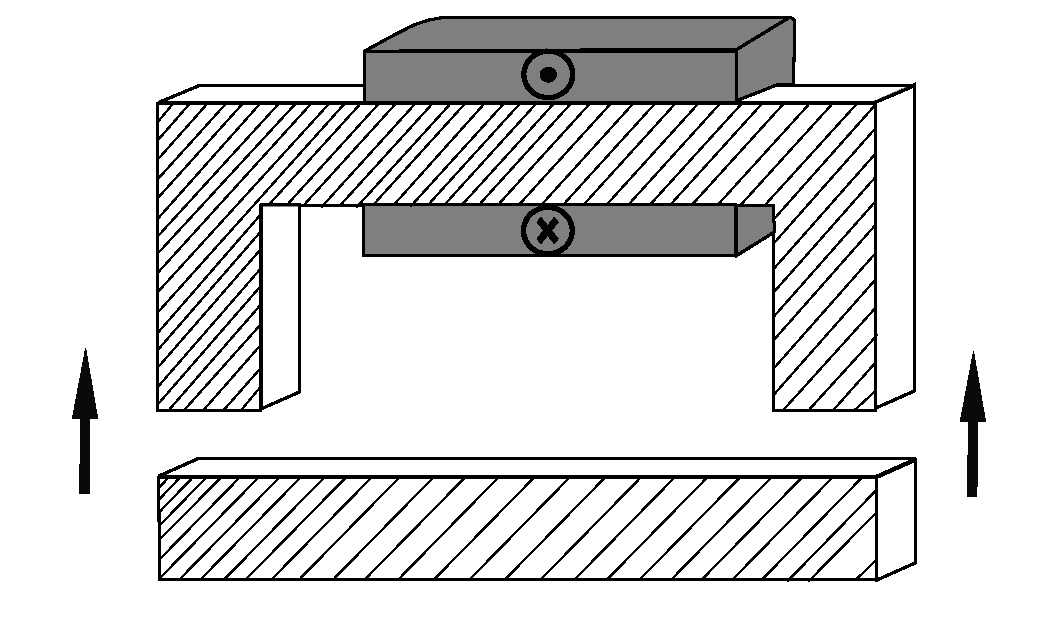
\includegraphics[width=\textwidth]{images/Capitulo_2/geometria_nucleo_radial}
        \caption{axial}
        \label{fig:geometria-axial}
    \end{subfigure}
    \caption{Geometrias de electroiman}\label{fig:geometria-electroimanes}
\end{figure}

\begin{figure}[htb]
    \centering
    \begin{subfigure}[b]{0.4\textwidth}
        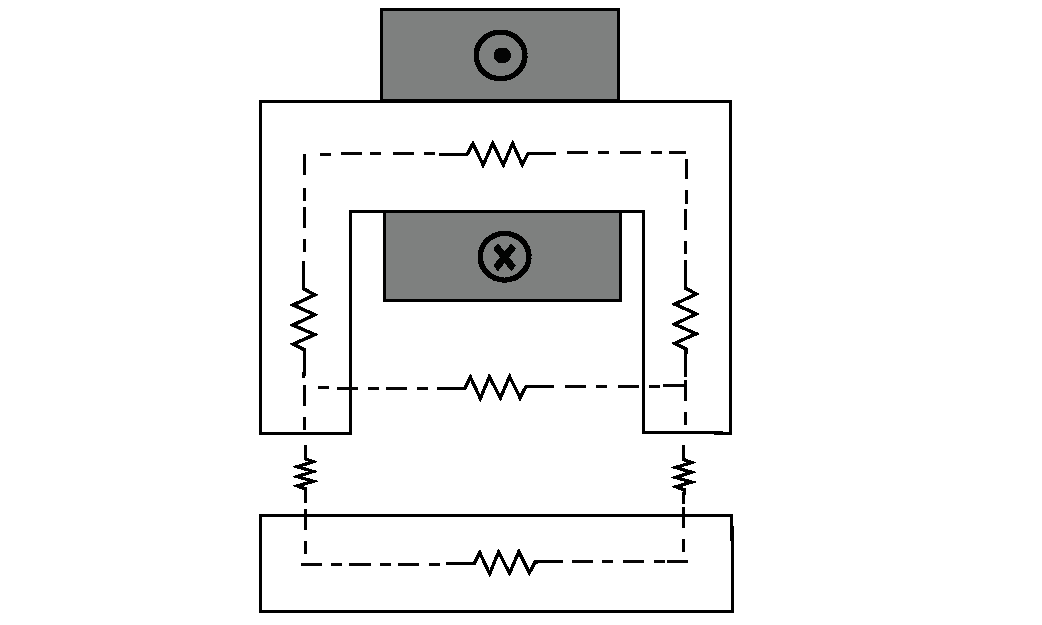
\includegraphics[width=\textwidth]{images/Capitulo_2/modelo_reluctancias_eir}
        \caption{radial}
        \label{fig:geometria-radial}
    \end{subfigure}
    ~ %add desired spacing between images, e. g. ~, \quad, \qquad, \hfill etc. 
      %(or a blank line to force the subfigure onto a new line)
    \begin{subfigure}[b]{0.4\textwidth}
        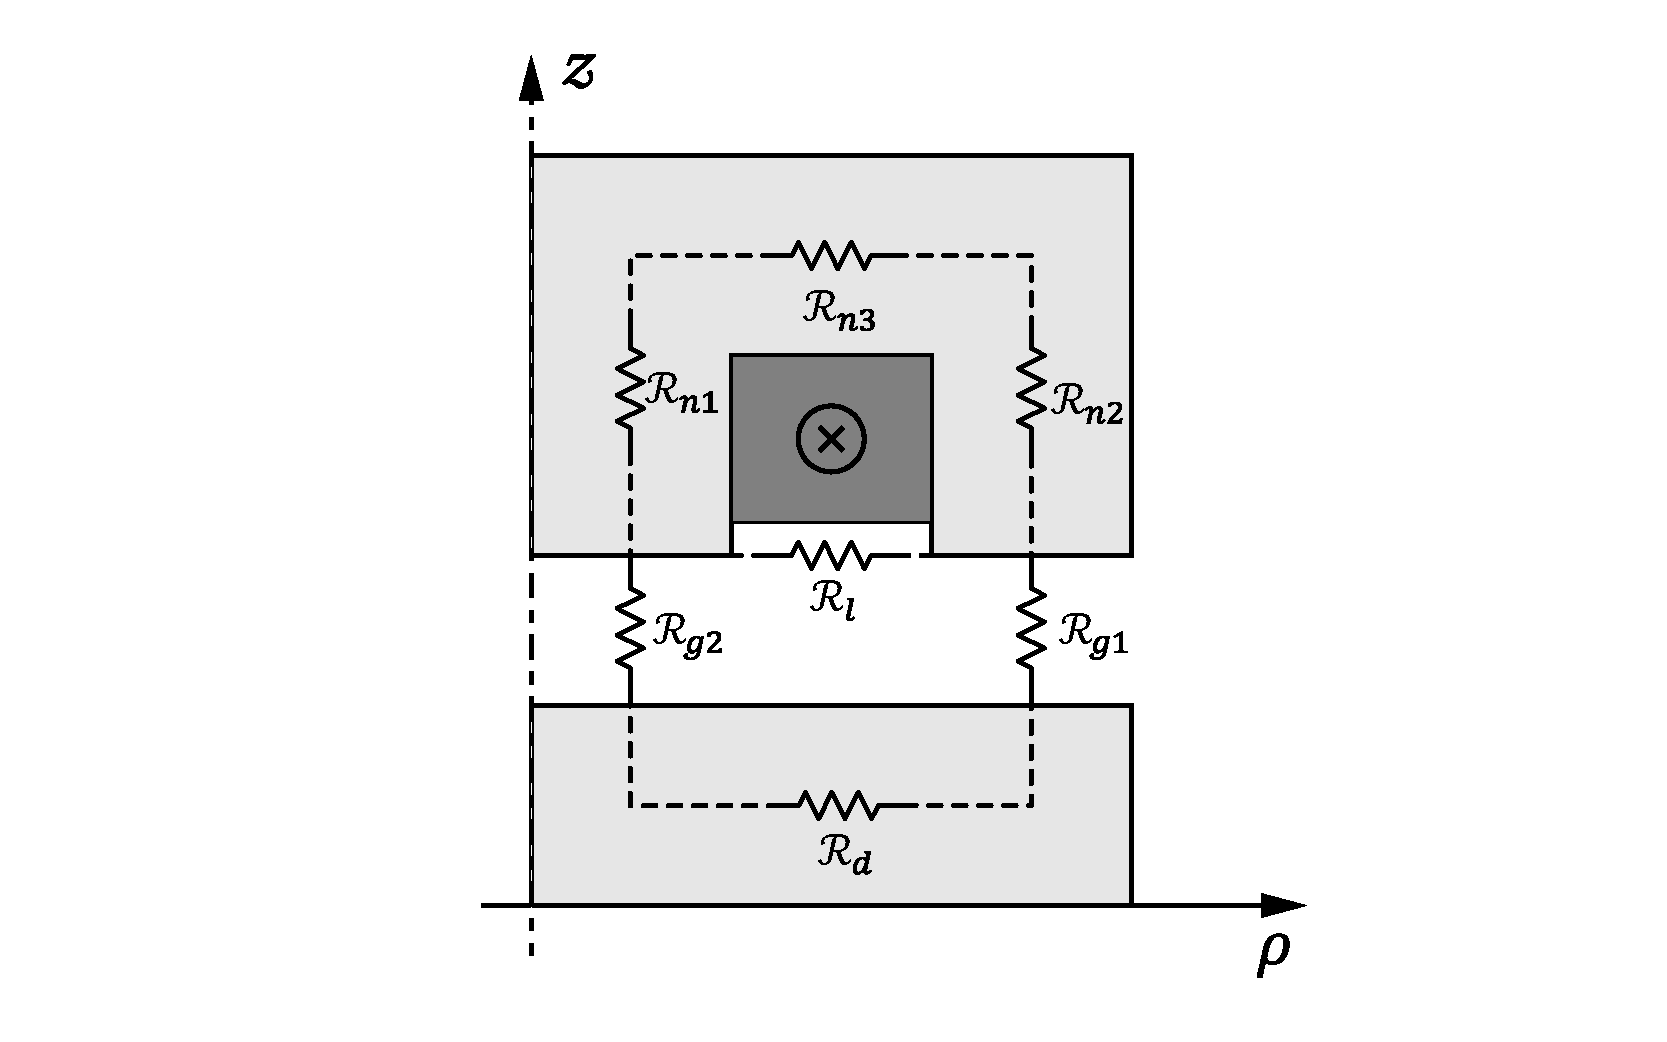
\includegraphics[width=\textwidth]{images/Capitulo_2/modelo_reluctancias_eia}
        \caption{axial}
        \label{fig:geometria-axial}
    \end{subfigure}
    \caption{Modelo de reluctancias}\label{fig:geometria-electroimanes}
\end{figure}

El electroiman posee una geometria como la de la figura ??, aplicando el analisis de circuitos magneticos el sistema se pude modelar como el circuito de reluctancias de la figura ??. Entonces la reluctancia total del circuito puede escribirse como
\begin{equation}
	R = ???
\end{equation}
Si consideramos los terminos ?? y ?? como insfinificantes entonces la fuerza se puede expresarse como:
\begin{equation}
	F = ???
\end{equation}
Esta ecuacion puede encontrarse en la literatura ??,?? y ??, para llegar a esta ecuacion fue necesario hacer varias suposiciones como despreciar flujo de fluga, el efecto marginal, y que la reluctancia del nucleo es mucho menor a la reluctancia del gap, estas condiciones podrian cuplirse en otros sistemas pero caso de un rodamiento magnetico no.

Si ponemos a prueba  la ecuciones con valores de A,B,y D  resulta en una fuerza de ?? newtons, en cambio si realizamos simulacion en FEM, para el mismo sistema, la simulacion arroja un valor de N.

Si reescribimos la ecuaion ?? pero esta vez sin ignorar los terminos ?? correspondientes a nucleo del electroiman, obtenemos la ecuacion ??
\begin{equation}
	F = ???
\end{equation}
Sustituyendo los valores usados anteriormente, la ecuacion nos arroja una fuerza de ?? newtons. La fuerzas coincide entre la simulacion FEM y las ecuacion que habria sido usada para calcular los electroimanes.

Para un electroiman axisimetrico donde la goemtria cumple condiciones de xx, xx. calculamos una fuerza xx N, sin embargo la simulacion FEM nos arroja un valor de xx.

Al observar el flujo magnetico podemos ver como el campo magnetico se curva en los extremos del iman, a esta distorsion en las lineas de campo magnetico debido a las discontinudades del medio se le conoce como flujo marginal.

Entonces para el correcto modelado del electroiman necesitamos incluir los efectos del flujo marginal en nuestro modelo.

En [??] se presenta un nuevo metodo para modelar la reluctancia de un entrehierro, para la geometria del electriman a) el entrehierro se puede modelar como b??) y para la geometria del electroiman axisimetrico el entrehierro se puede modelar como??, incluyendo estos nuevos valores en el modelo del reluctancia que conciden con la simulacion fem.

Ahora que tenemos un modelo adeacuado para la fuerza de los electrimanes, es necesario un procecidimiento para dise�arlos.

A partir de la ecuacion ??  podemos observar podemos varariar ?? parametros a la hora de dise�ar un electriman, idealmente queremos el electriman mas peque�o y que consuma menos corriente, y que pueda ejercer la fuerza que necesitemos $F$ a una distancia $d$.

Empezando por los terminos de fuerza magnetomotriz, para un electriman peque�o incrementarios el termino NI y una area transversal muy peque�a, sin embargo, esta condiciones causaria la saturacion del nucleo. lo cual no solo insertaria mas no-linealiadades dentro del sistema, si no que tambien generaria mayores perdidas.

Para evitar saturar el nucleo entonces tenemos que limitar la induccion magnetica a la que sometemos el nucleo, reordenando la ecuacion de ??, podemo determinar la induccion maxima de la forma:

\begin{equation}
	(NI)_{max} =  \frac{\phi}{A}
\end{equation}

El valor $NI_{max}$ solo depende de la logitud del entrehierro y del punto de saturacion del nucleo del electriman, esto implica que materiales con un punto de saturacion mas alto son mejores para aplicaiones de electrimanes. 

Conociendo ahora la $F_{MM}$ maxima que podemos aplicar el nucleo, solo nos queda variar el area transversal para generar la fuerza requerida $F_max$ mediantes la formula ??

Falta ahora determinar los valores de $N$ e $I$, la relacion de estos dos terminos es de suma importancia, ya que ambos determinan las caracteristicas electricas del electriman definidas por los terminos de inductancia y resistencia, la inductancia como se vera mas adelante limitara la respuesta en frecuencia de los electroimanes mientras que la resistencia determinara la eficiencia.

La resistencia de la bobina del electroiman esta dada por
\begin{equation}
R = ??
\end{equation}
donde $l$ es la logitud promedio de una espira, $A$ es la seccion tranversal el conductor, $\sigma$ y N es el numero de vueltas

las perdidades por efecto joule en un electroiman estan dadas por
$W = I^2R$ 

Teniedo en consideracion todo lo anterior podemos resumir le proceso de dise�o de un electriman en los siguientes pasos

\begin{enumerate}
\item Determinar condiciones de operacion y, v, $f_{max}$, $F_{max}$, $W_{loss_max}$ 
\item Seleccion de material
\item Calcular $NI_max$
\item Calcular A
\item Calcular $L_max$
\item Determinar Determinar I y N
\end{enumerate}

\subsection{Electroiman Radial}
\todo[inline]{Teniendo las condiciones de operacion, las cuales se sacan a partir de las condiciones de los papers}
\todo[inline]{Usando la herramienta arrojan los resultados siguientes}
\todo[inline]{Simulando en femm obtenemos los resultados}
\todo[inline]{Las dimensiones finales del subsistema son ?? son}
\todo[inline]{Los resultados estan dentro de los parametors aceptables, y las simulacion y los calculos del software conduerdan}
\subsection{Electroiman Axial}
\todo[inline]{Teniendo las condiciones de operacion, las cuales se sacan a partir de las condiciones de los papers}
\todo[inline]{Usando la herramienta arrojan los resultados siguientes}
\todo[inline]{Simulando en femm obtenemos los resultados}
\todo[inline]{Las dimensiones finales del subsistema son ?? son}
\todo[inline]{Los resultados estan dentro de los parametors aceptables, y las simulacion y los calculos del software conduerdan}
\subsection{Accionamiento de los electroimanes}
Ahora sabemos las caracteristicas de los electroimanes, necesitamos de un circuito para controlar la corriente que circula por la bobinas, en la seccion ?? hablamos  sobre las caracteristicas del circuito, y para el dise�o de los electroimas tuvimos que comprometernos los valores de alimentacion y respuesta en frecuencia, 

Un amplificador que opera un modo lineal como el de la figura?? opera de la siguientemanear, supongamos que tenmos que hacer pasar una corriente de ?? amperes a traves de una carga de ?? ohms,  para que existan ?? amperes  se necesitan ?? volts, si nuestra fuente es de ?? volts esto implica que el transistor debe de absober los ?? restantes. Esto implica disipar ?? W de potencia en forma de calor. Entonces es evidente la baja eficiencia de operar en este modo.

En cambio si en lugar de trabajar en la region lineal del transistor decidimos operar en las zonas de saturacion corte, la disipacion de energia en forma de calor es mimina, para controlar la corriente que circula comuntamos entre un estado a otro de manera que el promedio de la corriente sea la corriente deseada.

En la practica estos switches son implemetados usando transistores, en especial transistores MOSFET debido a su baja resistencia en encendido Ron.

El mosfet es un dispositivo que controla la corriente a traves del voltaje aplicado en sus temrinales. donde la relacion entre estas se encuntra determinada por

\begin{equation}
I_d = G(V_g - V_{th})^2
\end{equation}

Donde $V_{th}$ conocido como voltaje de treshhold es volaje minimo para activar el transistor. Una vez el voltage de compuerta $Vg$ llega sobrepasa el valor $V{sat}$ el transistor no puede dejar pasar mas corriente y simplemente se comparta como un ressitencia de valor $R_{on}$ a esta modo de operacion se le conoce como saturacion.

Cuando se trata de conmutar una carga inductiva se generan picos de voltaje, la corriente que circula por un inductor instantanea o discotinua, es por eso que se necesitan de un diodo, para que lo corriente logre recircular y disminuir de manera controlada, para es circuito de la figura ?? la corriente disminuye en una razon de $-L/V_d$

El problema ahora es que el incremento y decremento en la corriente actua de forma asimetrica, debido a que el cambio de la corriente depende del voltaje aplicado seria necesario aplicar un voltaje inverso, para eso es necesaria una configuarion como la mostrada en figura ??

Esta configuracion es comunmente conocida como puente H y presenta varios detalles para implementacion, el primero de estos es la  activacion de los transistores, como ya se ha mencionado antes para operar de la manera mas eficiente es necesario llevar los trasistores a su punto de saturacion, en la mayoria de los trasistres de potencia este valor se encutra entre los 10 y 15 volts, dado que la mayoria de los circuitos de control operan entre 5 y 1.8 es necesario de un circuito extra para elevar el voltaje, no hacer esto terminaria en polarizar los trasistores en su zona lineal lo que resltaria en el calentamiento de  estos y baja eficiencia. 

Otro problema polarizar los trasitore ?? y ??, ya que para su correcta activacion es necesario un voltaje de hasta $V_{cc} + V{sat}$, ambos problemas son resulta mediante el uso de un circuito conocido como gate driver, donde su usa un arreglo de transtores, diodos y capacitores para proveer los voltajes correctos en las compuertas de los transistores sin nececidad de una fuente separada.

Podemos definir ahora dos estados de operacion del puente H, un modo de accionamiento, donde se incrementa o decrementa la corriente que circula en la bobina, y un modo de reeciclacion, donde la corriente se mantiene a un nivel casi constante, y donde solo estan presentes la perdidas ohmicas causadas por $R_{ESR}$ y $R_on$

Esta logica de operacion puede implementarse usando el circuto de la figura ??, donde el arreglo de comparadores y flip flops permite controlar la corriente con una precision del $xx\%$

Como ya se ha mencionado, la razon de cambio de un inductor esta limitador por su inductancia y el voltaje aplicado en sus terminales con una magnitud de xx, esto implica que si tratamos de generar  una se�al senoidal, la frecuencia maxima que podriamos generar sin distorsionar la se�al seria seria

\begin{equation}
\frac{di}{dt}_{max} = 2 \pi f_{max} A = \frac{L}{V} 
\end{equation}

depejando la frecuencia maxima tenemos
\begin{equation}
f_{max} = \frac{L}{2 \pi V A} 
\end{equation} 
Donde podemos ver la frecuencia maxima de la se�al de salida depende de la amplitud de la misma, esta condicion  conocida como "slew rate limiting" es un fenomeno comun en los amplificadores y basta con conocer los limites de operacion del dispositivo para evitar tal operacion.

\begin{figure}[htb]
    \centering
    \begin{subfigure}[b]{0.4\textwidth}
        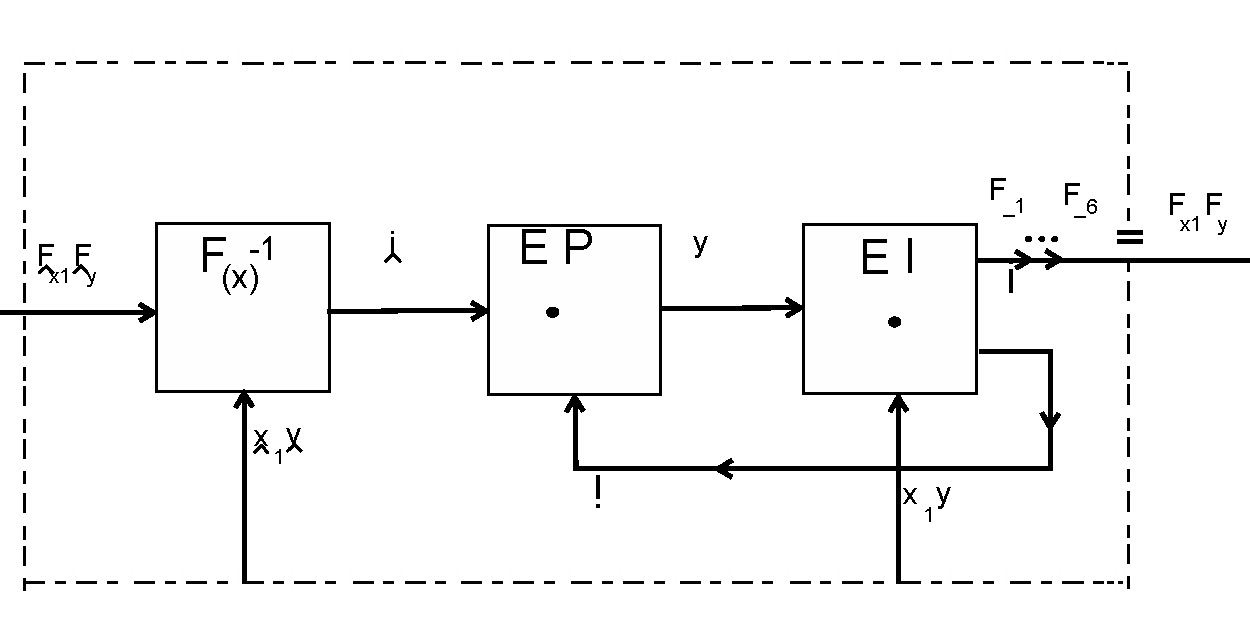
\includegraphics[width=\textwidth]{images/Capitulo_2/fb_linearization}
        \caption{Esquema de retroalimentacion}
    \end{subfigure}
    ~ %add desired spacing between images, e. g. ~, \quad, \qquad, \hfill etc. 
      %(or a blank line to force the subfigure onto a new line)
    \begin{subfigure}[b]{0.4\textwidth}
        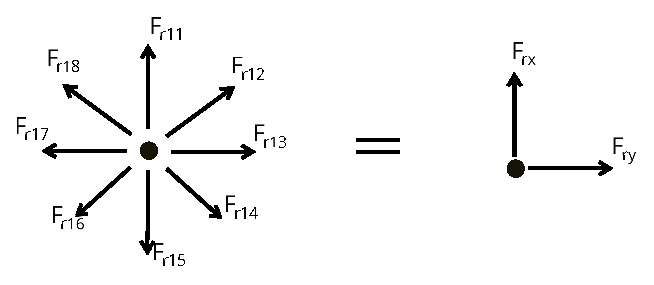
\includegraphics[width=\textwidth]{images/Capitulo_2/ferzas_radial}
        \caption{Equivalencia de fuerzas}
    \end{subfigure}
    \caption{Linearizacion de electroimanes}
\end{figure}



En caso de operar mas alla del limite se presenta una atenuacion de magnitud
\begin{equation}
A = \frac{L}{2 \pi V f} 
\end{equation} 
esta atenuacion concide con la de un filtro de pasabajas de primer orden, con frecuencia de corte $f_max$ y una caida de $20dB$ por decada, para los electrimanes presentados en ?? esta respuesta corresponde a las graficas de la figura ??. 

\section{M�dulo de Compensaci�n para Cargas Est�ticas}
Para la fuerza y por tanto la corriente que debe de suministrar los electroimanes se introduce el modulo de de compensacion para cargas estaticas, este modulo consisten en 3 partes, un iman permanente, un nucleo ferromagnetico para guiar el campo, un mecanismo para cambiar la posicion y por tanto la fuerza, un motor electrico, y un circuito para controlar la posicion del motor.

A partir de la ecuacion ?? sabemos que la fuerza que ejerce un electroiman pasivo esta dada por su valor Hc, Br, y las dimensiones del iman, done los valores Hc,Br dependen del material del que esta compuesto, y el punto hasta donde fue magnetizad.

Respecto a las dimension, un iman con una gran seccion transversal producira mas fuerza de una manera proporcional, mientras que incremetar su logitud solo incrementara la fuerza de manera logaritmica.

Es nuestro objetivo en este caso dise�ar electroiman-nucleo mas peque�o posible, debido a que las dimensiones de electroimanes y composicion de los imanes permantes estan dadas por el fabricante nos limitamos a seleccionar el iman mas peque�o disponible que generara al menos una cantidad $F_min$ de fuerza estando en la configuracion xx.

Las dimensiones del nucleo se seleccionan de tal manera que el iman pasivo pueda se acomodado dentro de este.

Para el dise�o del mecanismo tenemos el siguiente proceso
\begin{enumerate}
\item Especificar $F_{max}$, $y_{min}$
\item Seleccionar el iman con el $H_c$, $B_r$
\item Seleccionar las dimensiones segun la tabla ??
\item Dimensionar el nucleo guia de manera que acomode correctamente el iman passivo
\item Usar la formula ?? Calcular la fuerza $F_{max}$.
\item Si la fuerza $F_{req} > F_{im}$ incrementar las dimension y repetir los pasos.
\end{enumerate}

Asi como se hizo en la seccion ??, podemos validar nuestro modelo mediante una simulacion FEM, los que resulta en la siguiente grafica.

\begin{figure}[htb]
\begin{center}
\centering
\missingfigure[figwidth=8cm]{Fuerza del iman pasivo}
\caption{Fuerza del iman pasivo}
\end{center}
\end{figure}


\todo[inline]{Software para el calculo del iman passivo}
\todo[inline]{Simulacion verificacion del iman passivo}
\todo[inline]{Caraterizacion dela fuerza del iman passivo}
\todo[inline]{Modelo del mecanismo}
\todo[inline]{Acionamiento de sistema}
\todo[inline]{Caracteristicas dinamicas}
\section{Sensores Capacitivos de Desplazamiento}
\subsection{Electrodos}
El elctrodo es la parte fundamental del SCD, y su geometria afecta de manera directa a la sensitivadad del dispositivo.

Modelar la relacion entre la geometria del sensor y su sensitividad requiere solucionar la ecuacion.
\begin{equation}
ecuacion de poisson para medio discontinueo
\end{equation}

Las soluciones de esta ecuacion estan fuerza del alcanze de este trabajo, asi como se hace [??] nos disponemos usar el simulador electrostatico de FEMM para determinar la configuracion optima.

El electrodo del SCD posee una geometria de forma
\begin{figure}[htb]
\begin{center}
\centering
\missingfigure[figwidth=8cm]{Geometria del SCD}
\caption{Geometria del SCD}
\end{center}
\end{figure}
donde $d_i$ es el diametro externo del electrodo positivo, $d_o$ es el diametro interno del electrodo positivo, la relacion entre las area de ambos electrodos es $\alpha$

Si relizamos una simlacion en barrido, variando los parametros podemos observar que, entres mas grande sea el area del electrodo mas grande es capacitancia, esto se podia esperar observando la ecuacion del capacitor ??. 
Dado un diametro total $D$ el valor de $\alpha$ que maximiza la capacitancia del sensor es 1, o en otras palabras, areas iguales del anillo interior y exterior.

Calcular los parametros que maximizan la capacitancia, consideramos funcion escalar $f(\vec{P})$ el gradiente $\nabla f$ es el vector que indica el mas rapido incremento de la funcion f, asi pues si calculos de manera iterativa el vector de parametros p de la forma

\begin{equation}
\vec{P}_{k+1} = \vec{P}_k + \gamma \nabla f
\end{equation}

el vector de parametros $\vec{P}$ terminara por converger en el maximo local, de la fucion $f$, este metodo es conocido como descenso por gradiente.

Para su implemtacion, usamos un script capaz de generar una configuracion del sistema, usar femm para calcular su capacitancia, y de manera descrita calcular las derivadas, y de manera iterativa llegar los parametros que optimizan la sensitividad.


\todo[inline]{Descripcion de los efectos de la geometria en los sosores de capacitancia proyectada}
\todo[inline]{Simulacion femm}
\todo[inline]{Software para calculo de geometria optica}
\todo[inline]{Dimensiones finales del sensore}
\todo[inline]{Caracteristicas finales del sensores}
\subsection{Circuito de acondicionamiento}
\todo[inline]{Conversion de capacitancia a frecuencia}
\section{Integracion}
Para la correcta simulacion y control de se requiere de las ecuaciones que describan la dinamica del rotor.

\begin{figure}[htb]
\begin{center}
\centering
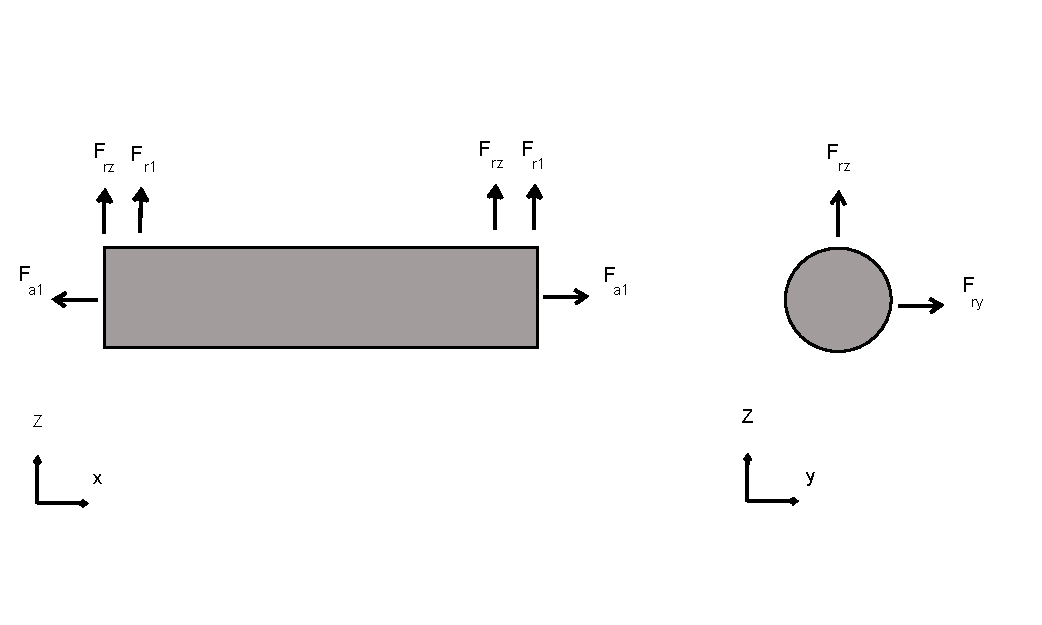
\includegraphics[width=12cm]{images/Capitulo_2/diagrama_cuerpo_libre_rotor}
\caption{Diagrama de cuerpo libre del rotor}
\label{fig:control:inercia-rmh}
\end{center}
\end{figure}
Los electroimanes radiales Fr1 y Fr2 ejercen fuezas en el plano z,y, mientras que los electroimanes axiales ejercen fuerzas en el ejex, y el iman permanente ejerce fuerzas en el eje z.
\begin{equation}
	\vec{F}_{r} = \begin{pmatrix}
	0\\
	F_{ry}\\
	F_{rz}\\
	\end{pmatrix}
	\vec{F}_a = \begin{pmatrix}
	F_{ax}\\
	0\\
	0\\
	\end{pmatrix}
	\vec{F}_p = \begin{pmatrix}
	0\\
	0\\
	F_{pz}\\
	\end{pmatrix}
\end{equation}
Los respectivos momentos son
\begin{equation}
	\vec{M}_r = \vec{r}_r \times \vec{F}_r 
\end{equation}
Existe un problema con simplificar la acci�n conjunta de los electroimanes axiales en xx, es posible ver que el momento generado cuando la fuerza es xx es xx, y el torque generado cuando la fuerza es xx va en el mismo sentido, entonces tenemos que el momento que ejerce los electrimanes raidales es
\begin{equation}
	\vec{M}_A = \vec{r}_a \times abs(\vec{F}_a)
\end{equation}

\begin{figure}[htb]
\begin{center}
\centering
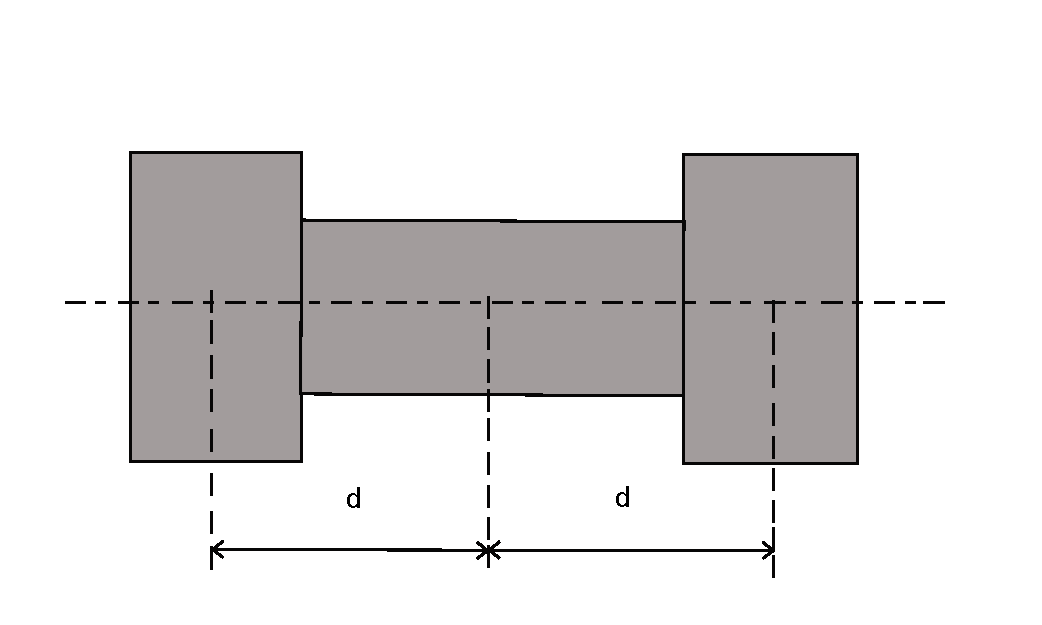
\includegraphics[width=12cm]{images/Capitulo_2/diagrama_momentos}
\caption{Momentos de inercia}
\label{fig:control:inercia-rmh}
\end{center}
\end{figure}


Para la matriz de inercial podemos diferencia la barra de los collarines de levitaci�n como se muestra en la figura \ref{fig:control:inercia-rmh} y aplicando el teorema de ejes paralelos podemos reescribir su matriz de inercia como
\begin{equation}
	[I] = \begin{pmatrix}
	I_{xxa} + 2I_{xxb}  & 0 & 0\\
	0 & I_{yya} + 2I_{yyb} + 2m_b r_b^2 & 0\\
	0 & 0 & I_{zza}+2I_{zzb}+ 2 m_b r_b^2
	\end{pmatrix}
\end{equation}
gracias a la simetr�a radial del cuerpo eje-collar�n los momentos principales $Iyy$ e $Izz$ son iguales, pudiendo reducir la ecuaci�n xx a la forma 
\begin{equation}
	[I] = \begin{pmatrix}
	I_{xx}  & 0 & 0\\
	0 & I_{\rho}  & 0\\
	0 & 0 & I_{\rho}
	\end{pmatrix}
\end{equation}
permitimos la libre rotacion dentro del eje x del marco de referencia movil
la velocidad angular es xx, entonces se tiene que
\begin{equation}
  \omega = \omega_\phi +
   \Omega
\end{equation}
calcular el producto cruz requiere que ambos vectores esten en el mismo marco de referencia asi que transformamos los vectores de fuerza al marco movil usando la transforamcion $T^{M}_O$
\subsection{Modelo dinamico del rotor}
\todo[inline]{Modelo del eje}
\todo[inline]{Modelo completo del sistema}
\subsection{Controladores}
\todo[inline]{Observador de estados}
\todo[inline]{Estabilzacion}
\todo[inline]{Servocontrol}
\todo[inline]{Discretizacion}
\todo[inline]{Fusion de sensores}
\todo[inline]{El problema del ruido}
\todo[inline]{Integrar los datos de 3 sensores}
\todo[inline]{El aplicando el filtro de kalman}